% !TEX root = ../../thesis.tex

\chapter{Sensitivity of Building Properties and Use Types for the Application of Adaptive Photovoltaic Shading Systems}
\chaptermark{Sensitivity of Building Properties and Use Types}
\label{ch:asfArchetype}

\graphicspath{{chapters/ch3Archetype//Images/}}

\begin{chapterabstract}
AAn adaptive solar facade can improve building energy performance by controlling solar heat gains and natural lighting, while simultaneously generating electricity on site. The adaptive control of the solar facade is determined through an optimisation algorithm that minimises the net energy demand. This chapter first evaluates the sensitivity of the adaptive solar facade to the thermal performance of the building envelope for a south facing room in Zurich. Then the performance of an adaptive solar facade is evaluated on 11 building use types spanning six construction periods. In addition, the performance of an adaptive system is compared to an equivalent static photovoltaic system, and a facade with no shading system. Results show that the adaptive solar facade performs best in buildings that have a high cooling demand and low heating demand. This is because the optimum configurations for cooling minimisation generate the maximum photovoltaic electricity. Higher energy saving potentials are observed in newer buildings with low envelope thermal transmittance (U-value or infiltration). However, in buildings with a very high cooling demand, and no heating demand, there is only a small improvement in performance compared to an equivalent static system. An adaptive solar facade is therefore an optimum solution when there are both heating demands, and cooling demands present. Modern offices, retail stores, food stores, and schools have this property and perform well with an adaptive solar facade compared to an equivalent static system, and a facade with no shading.
\end{chapterabstract}

\blfootnote{Jayathissa, P., Zarb, J., Hofer, J. \& Schlueter, A. Sensitivity of Building Properties and Use Types for the Application of Adaptive Photovoltaic Shading Systems. Energy Procedia, Proceedings to CISBAT (2017)}

\newpage

\section{Introduction}
\label{ch:introduction3}
% !TEX root = 99_main.tex

The built environment is responsible for 19\% of global greenhouse gas emissions \cite{IPCC}. Fortunately, the use of existing technologies such as building integrated photovoltaics (BIPV), thermal insulation, and efficient building systems can mitigate up to 50\%-90\% of this emission portfolio \cite{IPCC}.\\

Thin film photovoltaics (PV) in particular have improved in terms of efficiency, cost, and light weight integration \cite{NREL, kushiya2014cis, kaelin2004low, jelle2012building}, which influenced the development of the adaptive solar facade (ASF) \cite{nagy2016adaptive}. The adaptive solar facade consists of an array of independently actuated photovoltaic panels that can move in two axes at a range of 90$^{\circ}$. An example of this technology was built at the House of Natural Resources at the ETH Zurich Campus as seen in Figure \ref{fig:introduction3}. Through the control of solar radiation, the ASF is capable of minimising the building energy consumption in terms of heating, cooling and lighting demands, while simultaneously generating electricity on site.\\

The optimum panel angles of the ASF are determined through a model control algorithm detailed in Chapter  \ref{ch:asfSimulation} \cite{jayathissa2017AE}. Simulations of building energy performance and photovoltaic electricity supply are performed for every possible combination of angles for each time step. Through an exhaustive search, the optimum combination is chosen. An ASF built on a  building with an inefficient heating system will tend to exist in a more open position in winter so that the room can heat naturally through solar radiation. Likewise, a building with an efficient heating system will tend to optimise more for the generation of electricity on site. This sensitivity to the building typology leads to an energy saving variation of 20\% - 80\% compared to an equivalent static system \cite{jayathissa2017AE, jayathissa2016PVSEC}. \\

This paper utilises the models proposed by in Chapter  \ref{ch:asfSimulation} to extend the evaluation to a variety of building archetypes in Zurich. We will first evaluate the sensitivity of the ASF performance to the envelope resistance, and infiltration. We will then evaluate 11 building use types spanning six construction periods from the the City Energy Analyst (CEA) for ArcGIS database \cite{fonseca2016city}. By doing so, we can evaluate the optimum building properties and types for the application of an ASF. \\


The remainder of the paper is organised as follows. The next section describes the simulation methodology. In Section \ref{ch:results3} we present the results of the case study which describes the sensitivity of the ASF to the building typology. Finally, Section \ref{ch:conclusion3} concludes the paper.

\begin{figure}
    \centering
    \begin{subfigure}[b]{0.47\textwidth}
        \includegraphics[width=\textwidth, trim= 0cm 0cm 0cm 12cm,clip]{honr.jpg}
		\label{fig:HoNR}
    \end{subfigure} \hfill
    \begin{subfigure}[b]{0.47\textwidth}
        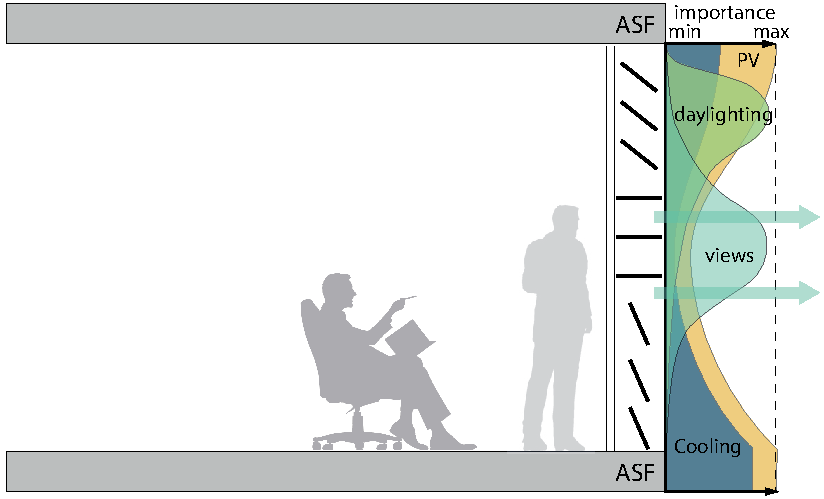
\includegraphics[width=\textwidth, trim= 0cm 0cm 0cm 0cm,clip]{facadeFunctionsnew.pdf}
		\label{fig:ASFschematic3}
    \end{subfigure}
    \caption{Left: An example of an ASF constructed at the House of Natural Resources. Right: a schematic describing how the facade can mediate solar radiation to optimise the internal environmental conditions \cite{nagy2016adaptive}}
    \label{fig:introduction3}
\end{figure}


% \begin{figure}
% \begin{center}
% \includegraphics[width=8cm, trim= 0cm 0cm 0cm 0cm,clip]{honr.jpg}
% \caption{An example of an ASF constructed at the House of Natural Resources \cite{nagy2016adaptive}}
% \label{fig:HoNR}
% \end{center}
% \end{figure}

% \begin{figure}
% \begin{center}
% 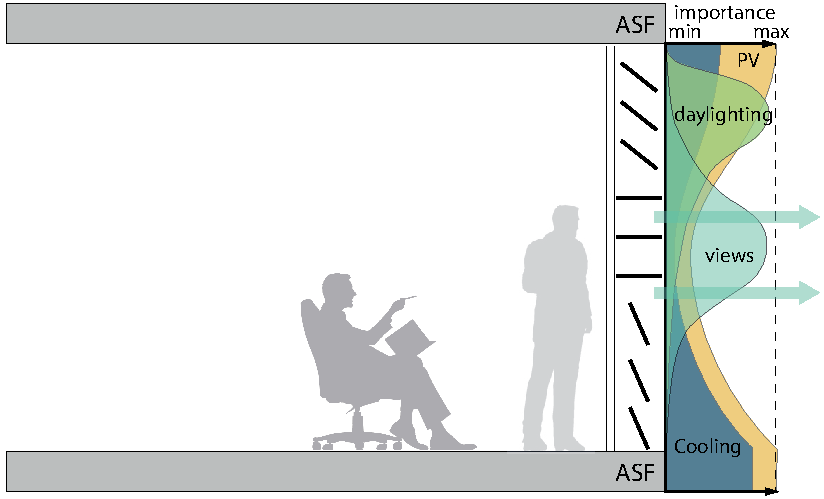
\includegraphics[width=8cm, trim= 0cm 0cm 0cm 0cm,clip]{facadeFunctionsnew.pdf}
% \caption{The facade acting as a mediator between the interior and exterior environment, while fulfilling various functions \cite{nagy2016adaptive}}
% \label{fig:ASFschematic3}
% \end{center}
% \end{figure}








\section{Methodology}
\label{ch:method3}
% !TEX root = 99_main.tex

A control methodology of adaptive photovoltaic shading systems to maximise PV electricity production while minimising the building energy consumption was proposed in Chapter \ref{ch:asfSimulation}. It will be briefly reviewed here for completeness.

\begin{itemize}
\item \textbf{Solar Radiation Model:} The radiation on the PV panels and window behind the ASF is calculated for a single configuration of the ASF using LadyBug/Radiance for a single time step of one hour \cite{roudsari2013ladybug,ward1994radiance}.
\item \textbf{PV Electricity Production:} The radiation result is coupled to an electrical circuit simulation of monolithically interconnected, thin-film CIGS PV modules. This model takes into account the effects of module self-shading and temperature dependence \cite{hofer2016parametric}.
\item \textbf{Building Energy Model:} A 5R1C single zone resistance-capacitance building model based on the ISO 13790 standard computes the heating or cooling demand of the building for the particular timestep \cite{de2008iso}. We assume that the only surface in contact with the external environment is the south facing glazed surface. All other surfaces are in contact with other thermal zones and modelled as adiabatic surfaces. The climate in Zurich is defined as an oceanic climate (Cfb) by the Koeppen Index with an average July temperature of 18.4$^{\circ}$C, and January temperature of 0.2$^{\circ}$C \cite{koppenZurich}.
% \added[id=pj, remark={may delete to trim to 6 pages}]{This will be further expanded in Section \ref{ch:rc}.}
\item \textbf{Daylighting Model:} A linear daylighting model based on the total flux methodology is used to determine the luminosity in the room \cite{szokolay1980handbook}. 
\item \textbf{Optimisation:} The simulation is conducted for all possible panel angle combinations. The angle combination with the lowest net energy consumption is chosen for each timestep.
\end{itemize}



% \subsection{Building Simulation Model}
% \label{ch:rc}

% \added[id=pj, remark={may delete to trim to 6 pages}]{This subsection describes the physics-based method to simulate the thermal behaviour of the building using a resistor-capacitor (RC) model. The model, shown in Figure \ref{fig:RC_Model}, consists of one internal thermal capacitance, and five thermal resistances.}

% \begin{figure}
% \begin{center}
%     \begin{circuitikz}[scale = 0.7, transform shape]
%       \draw (0,0)
%       node[label={left:$T_e$}] {}
%       to[short,*-] (1,0)
%       to[short] (1,1)
%       to[european resistor=$H_w$] (3,1); % The resistor

%       \draw(1,0)
%       to[short] (1,-1)
%       to[european resistor=$H_{em}$] (3,-1)
%       node[label={10:$T_m$}] {}
%       to[european resistor,l_=$H_{ms}$] (3,1)
%       node[label={10:$T_s$}] {}
%       to[european resistor,l_=$H_{is}$] (3,3)
%       node[label={10:$T_{air}$}] {}
%       to[european resistor,l_=$H_{ve}$] (1,3)
%       to[short,-*] (0,3)
%       node[label={left:$T_{sup}$}] {};

%       \draw(3,-1)
%       to[short,*-] (5,-1)
%       to[short] (5,1)
%       to[short,-*] (3,1);

%       \draw(5,1)
%       to[short] (5,3)
%       to[short,-*] (3,3)
%       to[european current source,l_=$\phi_{HC}$] (3,5);

%       \draw(5,1)
%       to[european current source,l_=$\phi_{sol}+\phi_{int}$] (7,1);

%       \draw(3,-1)
%       to[C=$C_m$] (3,-2)
%       node[ground]{};


%     \end{circuitikz}
%     \caption{\added[id=pj, remark={may delete to trim to 6 pages}]{A 5R1C Model of the single zone space \cite{de2008iso}}}
% \label{fig:RC_Model}
% \end{center}
% \end{figure}

% \added[id=pj, remark={may delete to trim to 6 pages}]{In this model, we assume that the only surface in contact with the external environment is the south facing glazed surface. All other surfaces of the room are in contact with other thermal zones of the building that we assume to hold the same room temperature. We therefore model them as adiabatic surfaces. Denoting by $T_m$, the temperature of the thermal mass in the room, the differential equation for the circuit in Figure \ref{fig:RC_Model} can be discretised as:}

% \begin{equation} 
% \label{eq:derivation}
%       T_{m_{k+1}}={\frac{\phi_{mtot}+T_{m_k}\Big(\frac{C_m}{\Delta t} - 0.5(H_{tr3}+H_e)\Big)}{\frac{C_m}{\Delta t} + 0.5(H_{tr3}+H_e)}}
% \end{equation}

\subsection{Sensitivity Analysis}

Sensitivities in the framework can be modelled by adjusting variables in the resistor-capacitor model. Two envelope sensitivities will be analysed in this study

\begin{itemize}

\item \textbf{Envelope Thermal Transmittance:} The building envelope is characterised in the RC model as $H_w$ which is the U-value of the envelope. 
\item \textbf{Infiltration:} The infiltration rate is modified as an air exchange conductance in the ISO RC model $H_{ve}$ detailed in Chapter \ref{ch:asfSimulation} \cite{de2008iso,jayathissa2017AE}.

This quasi-conductance is modelled as

\begin{equation} 
\label{eq:vent}
      H_{ve}= \frac{\rho c_a V_{room}}{3600}\Big[ ACH_{infl} + ACH_{vent}(1-\eta_{vent}) \Big]
\end{equation}

where: 

$\rho c_a$ is the heat capacity per air volume = 1200 $J/(m^3 K)$;

$\eta_{vent}$ is the efficiency of the ventilation heat recovery unit

$ACH_{vent}$ is the air changes per hour for ventilation of the room volume $V_{room}$

$ACH_{infl}$ is the air changes per hour for the infiltration of the room volume $V_{room}$ which is the variable in this sensitivity analysis

\end{itemize}


\subsection{Analysis of Archetypes}

Building envelope parameters are imported from the CEA Toolbox, an open source urban building simulation software. The archetype databases are publicly available on the CEA GitHub page \cite{CEAArchetypes,CEAToolbox}. From this data, the following variables are evaluated: envelope U-value, occupancy profile, human heat emissions, lighting control set point, lighting load, thermal set points, and building thermal capacitance.

One critical component not analysed in the evaluation is the window to wall ratio. This was kept constant to maintain a valid comparison.






\section{Results}
\label{ch:results3}
% !TEX root = main.tex

This section presents the results of the LCA analysis in relation to the 1) embodied  emissions, 2) a calculation of the emission factor, 3) sensitivity of the LCA to design and location, and 4) a comparison to other PV technologies.

\subsection{LCA of the Adaptive Solar Facade Manufacture}

A breakdown of six major midpoint impact indicators based of the ReCiPe methodology \cite{goedkoop2009recipe}  can be found in Figure  \ref{fig:embodied}. The largest embodied GWP contribution in the ASF comes from the solar panels, followed by the electronics and the supporting structure. The control and electronics systems play a large role in freshwater eutrophication, and human toxicity due to the high life cycle emissions of electronic systems.



\begin{figure}[H]
\begin{center}
\includegraphics[width=\textwidth, trim= 0cm 0cm 0cm 0cm,clip]{pieembodied}
\caption{Embodied emission breakdown of six major midpoint indicators. The solar panels, control/electronics, and steel frame have the highest life cycle impact}
\label{fig:embodied}
\end{center}
\end{figure}

\subsection{Calculation of GWP Emission Factor}
The combined GWP of main inputs to the ASF, previously described in Figure \ref{fig:BOS}, can be illustrated using a waterfall chart as shown in Figure \ref{fig:waterfall}. 


This gives us a final emission of 3037kgCO$_2$-eq. When the energy savings through adaptive shading is included in the system expansion, the final emissions come down to -8318kgCO$_2$-eq. Dividing these values by the photovoltaic electricity production over a 20 year life time of 9175kWh, an emission factor of 331gCO$_2$-eq/kWh is obtained for the system without adaptive shading and -906 gCO$_2$-eq/kWh with adaptive shading.


\begin{figure}[H]
\begin{center}
\includegraphics[width=\textwidth, trim= 0cm 0cm 0cm 0cm,clip]{waterfall}
\caption{Waterfall diagram of GWP of the ASF not including photovoltaic electricity production. When reading from left to right, the far left bar details the embodied carbon emissions. The second, third and fourth bar detail the actuation, maintenance, and disposal respectively. This leaves us with a final emissions value (grey bar) of 3037kgCO$_2$-eq. The orange bar details the emission reduction through adaptive shading which is part of the system expansion bringing the total down to -8318kgCO$_2$-eq. When these totals are divided by the photovoltaic electricity production (9174kWh) an emission factor of 331gCO$_2$-eq/kWh is attained for the system without adaptive shading and -906 gCO$_2$-eq/kWh with adaptive shading. Note that the waterfall chart itself doesn't show PV electricity generation. This is taken into account in the emission factor.}

\label{fig:waterfall}
\end{center}
\end{figure}



\subsection{Sensitivity Analysis}


The sensitivity analysis is shown in Figure \ref{fig:sens}. The performance of the ASF is dependent on the location where it is operated as explained in Section \ref{ch:Meth:Opp}. Changing the weather files of the simulation, and the electricity mix of the country brings interesting results. Geneva has a similar climate to Frankfurt, however the local electricity mix is dominated by hydro and nuclear power which has a very low GWP potential \cite{itten2012life}. This would then increase the emission factor of the ASF to 53.5 gCO$_{2}$-eq/kWh. This difference arises as the greenhouse gas emission savings of adaptive shading are dependent on the emission factor of the grid mix.
Spain on the other hand has a warmer climate, with higher solar radiation, but a less greenhouse gas intensive electricity mix. This ultimately results in a similar emission factor of the ASF of -825 gCO$_{2}$-eq/kWh.\\


A case without the actuators and necessary control system for a dynamic system is also presented. Instead, panels are optimally orientated at 45$^{\circ}$ to the horizontal axis. This reduces embodied greenhouse gas emissions by 12.1\% from the baseline highlighted in Figure \ref{fig:embodied}. However the reduction in electricity production, and savings through adaptive shading, result in a 15\% higher emission factor.\\

The choice of actuator has a small impact on the embodied carbon emissions. Changing a single Soft Robotic Actuator (including the air compressor, tubing, and maintenance) to a classical servo motor increases the total embodied GWP by 23\% from 2498 kg CO$_{2}$-eq to 3073 kg CO$_{2}$-eq. However, the servo motors have lower operational emissions and maintenance. Ultimately an ASF with servo motors has a 1.5\% higher emission factor. \\


The control system design should be carefully thought out due to the high embodied human toxicity, freshwater eutrophication and terrestrial acidification. However simplifying the actuation control electronics has a minimal effect as the majority of the emissions lie in the inverter, cables, and air compressor. In terms of GWP, there is a 0.3\% difference which is negligible.



\begin{figure}[H]
\begin{center}
\includegraphics[width=\textwidth, trim= 0cm 0cm 0cm 0cm,clip]{sens.pdf}
\caption{Sensitivity analysis of the emission factor including the HVAC impact of adaptive shading based on location, actuation system, and control system}
\label{fig:sens}
\end{center}
\end{figure}

\subsection{Comparison to existing PV technologies}

Comparison of the ASF to other PV technologies and the German electricity mix is highlighted in Figure \ref{fig:compPV}. This comparison is conducted in Frankfurt am Main with an average irradiation of 855 kWh/m$^2$/year.\

The blue bars detail systems with no added shading benefits. Here the ASF, a static optimally orientated facade as used in Figure \ref{fig:sens}, and three classical flat facade installations are presented.  
The orange bars detail the system expansion where the ASF is built over glazed surfaces which also bring energy savings to the building. Because the GWP savings through adaptive shading offsets the entire embodied GWP, we have a system with a negative emission factor.





\begin{figure}[H]
\begin{center}
\includegraphics[width=\textwidth, trim= 0cm 0cm 0cm 0cm,clip]{compPV.pdf}
\caption{Comparison of facade installations in Germany with an average facade irradiation of 855kWh/m$^2$/year.
The ASF is compared to an optimally orientated static facade, and classic flat facade mounted PV solutions. The orange bars include the system expansion of energy savings through adaptive shading.}
\label{fig:compPV}
\end{center}
\end{figure}





% \section{Discussion}
% \label{ch:discussion}
% \input{5_discussion}

\section{Discussion and Conclusion}
\label{ch:conclusion3}
% !TEX root = 99_main.tex

This chapter presents a practical PDE for the design and fabrication of kinetic architectural elements. The PDE is capable of combining the multiple fields of structural engineering, energy engineering, control engineering, industrial design and architecture into one uniform environment, allowing the designers to handle the complexities of a multidisciplinary project. 

The major advantage of this environment is the considerable decrease in time between design iterations. Traditionally each of the respective stakeholders in the project would work on their individual design, and then exchange information in a meeting. With the PDE, the meeting is transformed from an information exchange session, to a design session where all stakeholders can collaboratively influence the design and immediately see the necessary results.  With traditional methods, five design iterations would normally take a month, whereas with the PDE, this can be condensed to a few hours. The design environment also develops with the project allowing for new parametric inputs, or new outputs to be created. This can be easily done with collaborative software management tools such as git, a distributed version control system.

One disadvantage is the overhead required to manage a PDE. Like a BIM manager, a PDE manager is required and must have a careful overview of the software. As the software ultimately determines the final form of the design, any errors in the software can be detrimental to the final design. It was therefore necessary for all stakeholders to conduct a final independent analysis prior to the submission of the final design. 

One limiting factor in the design of the PDE is the computational time. The full annual energetic analysis, for example, may take six hours to solve. Simplifications were therefore made to accelerate this process during the design stage, and the full complex evaluation was conducted afterwards to validate the simplified model.

It is also important to determine what aspects of the design should be contained within the PDE and what should be designed with classical methods. Essentially, all aspects where there could be conflicts between the stakeholders were included in the PDE, whereas many of the design details, such as the mounting brackets to the building, can still be designed independently and imported into the PDE as a static object. Over time, some static objects, such as the cantilevered bracket of the PV module became parametrised. 

Ultimately, this chapter presents a further step in the field of performative design by showing how a system as complex as a kinetic photovoltaic envelope, can be developed, prototyped and finally fabricated by a small team of four designers. The methodology can be utilised for any building component where multiple technological branches are required.




% \dictum[James C. Maxwell]{%
%   The true logic of this world is in the calculus of probabilities. }%
% \vskip 1em

% \Citet{Maxwell1865} derived some very useful equations for electromagnetic
% fields:
% \begin{align}
%     \nabla \cdot \vec{D} = \rho \\
%     \nabla \cdot \vec{B} = 0 \\
%     \nabla \times \vec{E} = -\frac{\partial \vec{B}}{\partial t} \\
%     \nabla \times \vec{H} = \vec{j} + \frac{\partial \vec{D}}{\partial t}
% \end{align}

% The energy--momentum relation, \cref{eq:energy-momentum}, is one of \emph{my}
% important results:
% \begin{align}
%     E^2 = m^2 c^4 + (p c)^2 \label{eq:energy-momentum}
% \end{align}

% Write units like this: \u{5}{\micro\meter}.

% \begin{figure}
%   \caption{A lovely face.}
% \label{fig:some-figure}
% \includegraphics{\dir/figure.pdf}
% \end{figure}
